\begin{Example}[berkeley8]{Berkeley admissions}
The \ODS\ \pname{predict} from the logit model, \pname{admit = dept gender},
for the Berkeley data is shown partially in \outref{out:catberk2.2}.
Each of the $ 2 \times 6$ samples defined by the explanatory factors
\pname{dept, gender}
gives rise to three observations: two response probabilities and
one logit, distinguished by the variable \verb|_TYPE_|.
\begin{Output}[htb]
\caption{Output \Dset\ \pname{predict} from the logit model for Berkeley admissions (partial)}\label{out:catberk2.2}
\small
\verbatiminput{ch7/out/catberk2.2}
\end{Output}

%% one figure
\begin{figure}[htb]
  \centering
  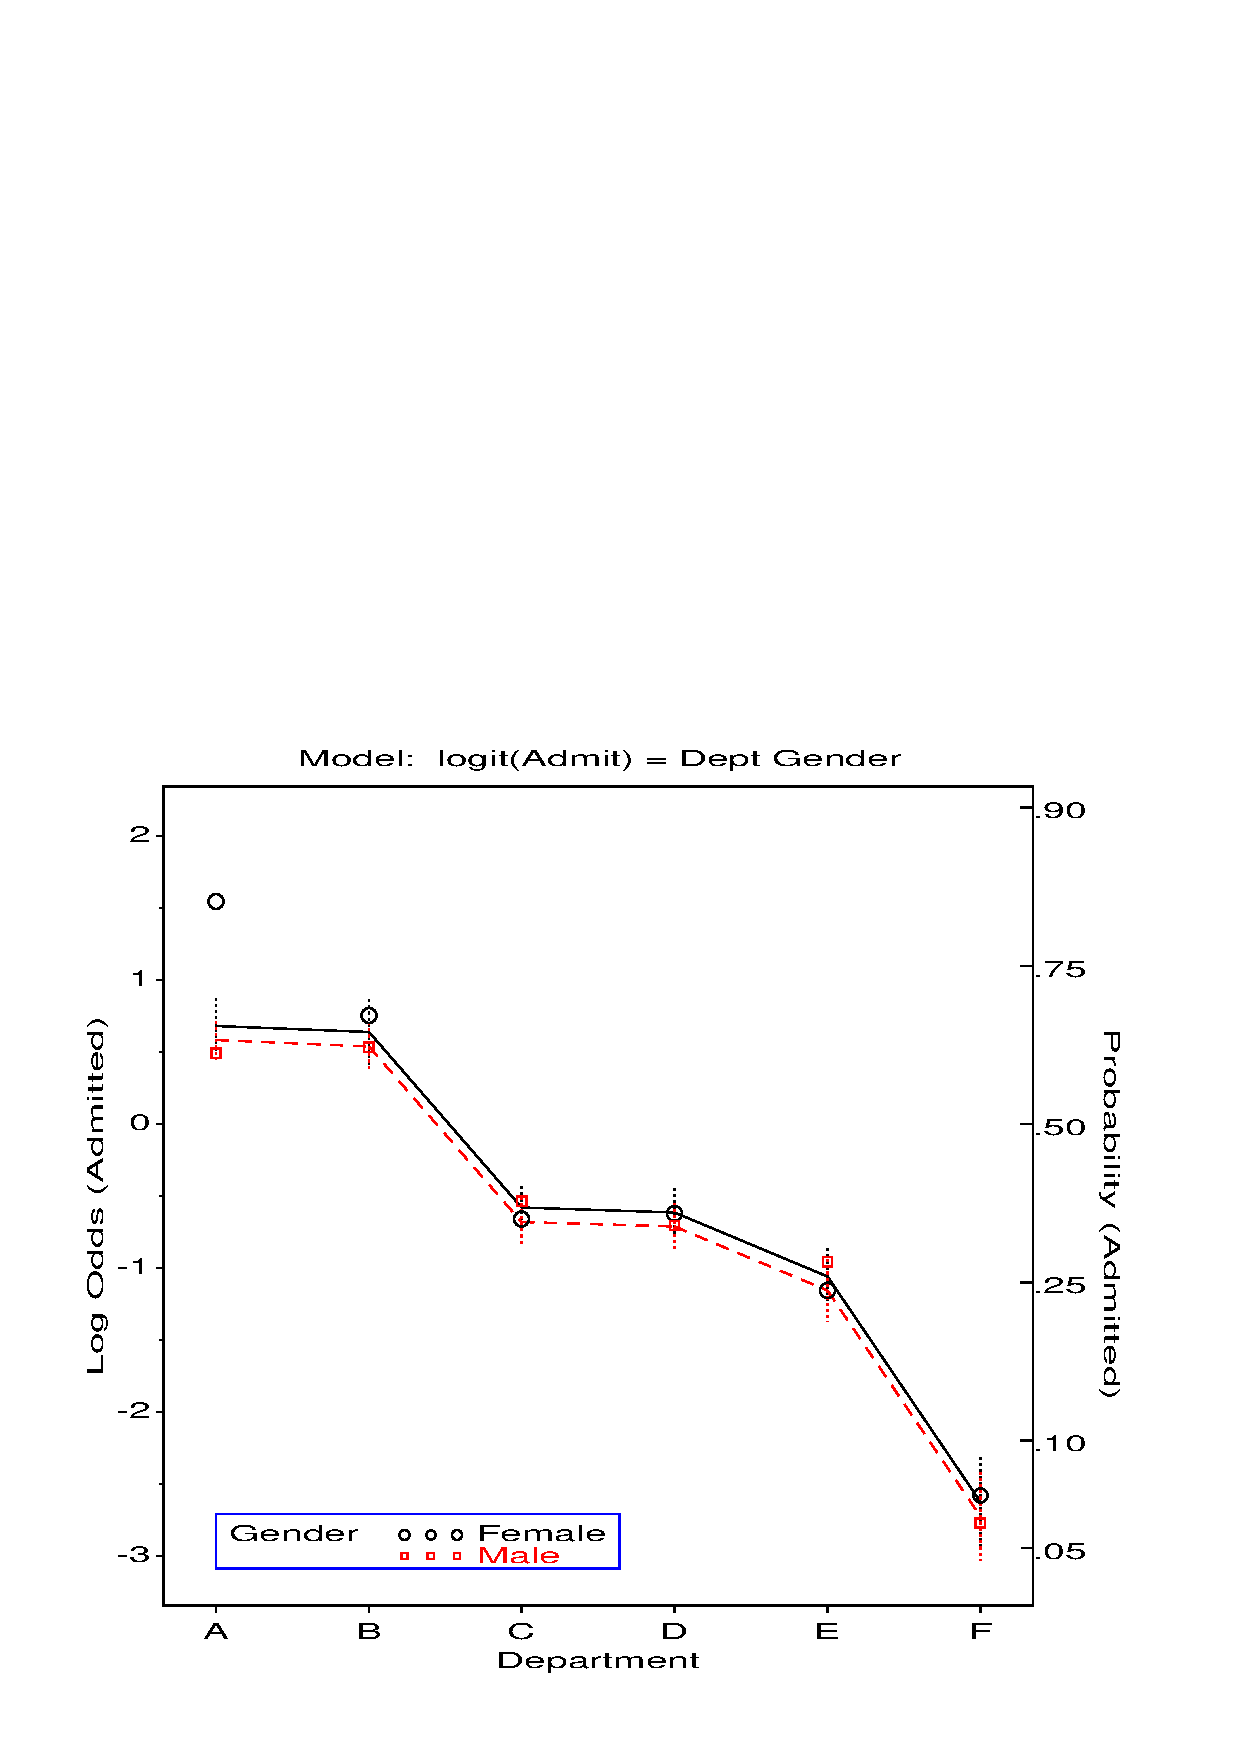
\includegraphics[scale=.6]{catberk2}
  \caption[Observed and fitted log odds of admission in the logit model]{Observed (points) and fitted (lines) log odds of admission in the logit model
  corresponding to [AD][AG][DG].  The error bars show individual 95\%
  confidence intervals around each fitted logit.}%
  \label{fig:catberk2}
\end{figure}

The statements below draw the plot of observed and predicted logits
(\verb|_type_='FUNCTION'|) shown in \figref{fig:catberk2}.
The \macro{PSCALE} constructs an \ADS\
which draws the probability values on the right vertical axis in the
plot.
The label for this axis is specified in the \stmt{TITLE}{GPLOT}, with
an angle, \pname{A=-90}, meaning the right-hand side, rotated \degree{90}.
By default, the macro uses the \pname{AXIS} and \pname{SYMBOL}
statements defined before the macro call.
Separate curves are
drawn for each level of the \pname{CLASS=GENDER} variable.
The values of the \pname{CLASS} variable may be labeled in the plot
or supplied in a \stmt{LEGEND}{CATPLOT}.
The parameter \pname{Z=1.96} specifies the multiple of
the standard error of the fitted logit (\verb|_SEPRED_|) used to
draw the error bars in the plot,
giving (asymptotic) 95\% individual confidence intervals.
\begin{listing}
%pscale(lo=-4, hi=3, anno=pscale, prob=%str(0.05,.1,.25,.5,.75,.9));

title h=1.6 'Model:  logit(Admit) = Dept Gender'
            a=-90 'Probability (Admitted)'
      h=3.5 a=-90 ' ';
legend1 position=(bottom inside left)  offset=(4,3)
        mode=share cborder=blue across=1
        shape=symbol(6,1.5) label=('Gender')
        value=(c=black 'Female'
               c=red   'Male');
axis1 order=(-3 to 2) offset=(4)
      label=(a=90 'Log Odds (Admitted)');
axis2 label=('Department') offset=(4);
symbol1 i=none v=circle h=1.7 c=black;
symbol2 i=none v=dot    h=1.7 c=red  ;
%catplot(data=predict,
   xc=dept, y=_obs_, class=gender,
   type=FUNCTION,
   z=1.96, anno=pscale, legend=legend1);
\end{listing}

The effects seen in our earlier analyses (Examples~\ref{ex:berkeley4}
and \ref{ex:berkeley4b})
may all be observed in this
plot.
The effect of gender is shown by the constant separation
between the two curves.
From the plot we see that this effect is very small and nonsignificant (compared
with the error bars).
If the gender effect were omitted from the model,
the fitted logits would be the same
for men and women applying to each department, and would plot as a curve
parallel to, but in between, the two shown in the graph.
Most of the observed points are quite close to their predicted values,
except in Department A,
where the probability of admittance for women is substantially
greater than that for men.
In \exref{ex:berkeley6} we dealt with this by allowing one extra parameter
for an association between admission and gender in department A,
giving the \loglin\ model \eqref{eq:berk2}.

We can see what this model ``looks like'' by recasting it in logit form.
The \loglin\ model \eqref{eq:berk2}
has an equivalent logit formulation, which also adds a 1 df term for an
effect of gender in department A,
\begin{equation}\label{eq:berk4}
  L_{ij} =
  \alpha   +  \beta _i^{\mbox{\scriptsize Dept}}
  +  \delta_{j=1} \beta^{\mbox{\scriptsize Gender}}
  \period
\end{equation}

This model may be fit
with \PROC{CATMOD} as shown below.  The association term between admission
and gender for Dept. A (\texttt{dept1AG}) is fit as a \pname{DIRECT}
variable.  The \pname{gender} variable is not included in the
\stmt{MODEL}{CATMOD}, so it must be listed in the
\stmt{POPULATION}{CATMOD}.
Because the \macro{CATPLOT}
uses the values in the \ODS, the plotting step is unchanged.

\begin{listing}
data berkeley;
   set berkeley;
   dept1AG = (gender='F') * (dept=1);

proc catmod order=data
            data=berkeley;
   weight freq;
   population dept gender;
   direct dept1AG;
   response / out=predict;
   model admit = dept dept1AG / ml noiter noprofile ;
%catplot(data=predict, xc=dept, class=gender, type=FUNCTION,
   z=1.96, legend=legend1);
\end{listing}

%% one figure
\begin{figure}[htb]
  \centering
  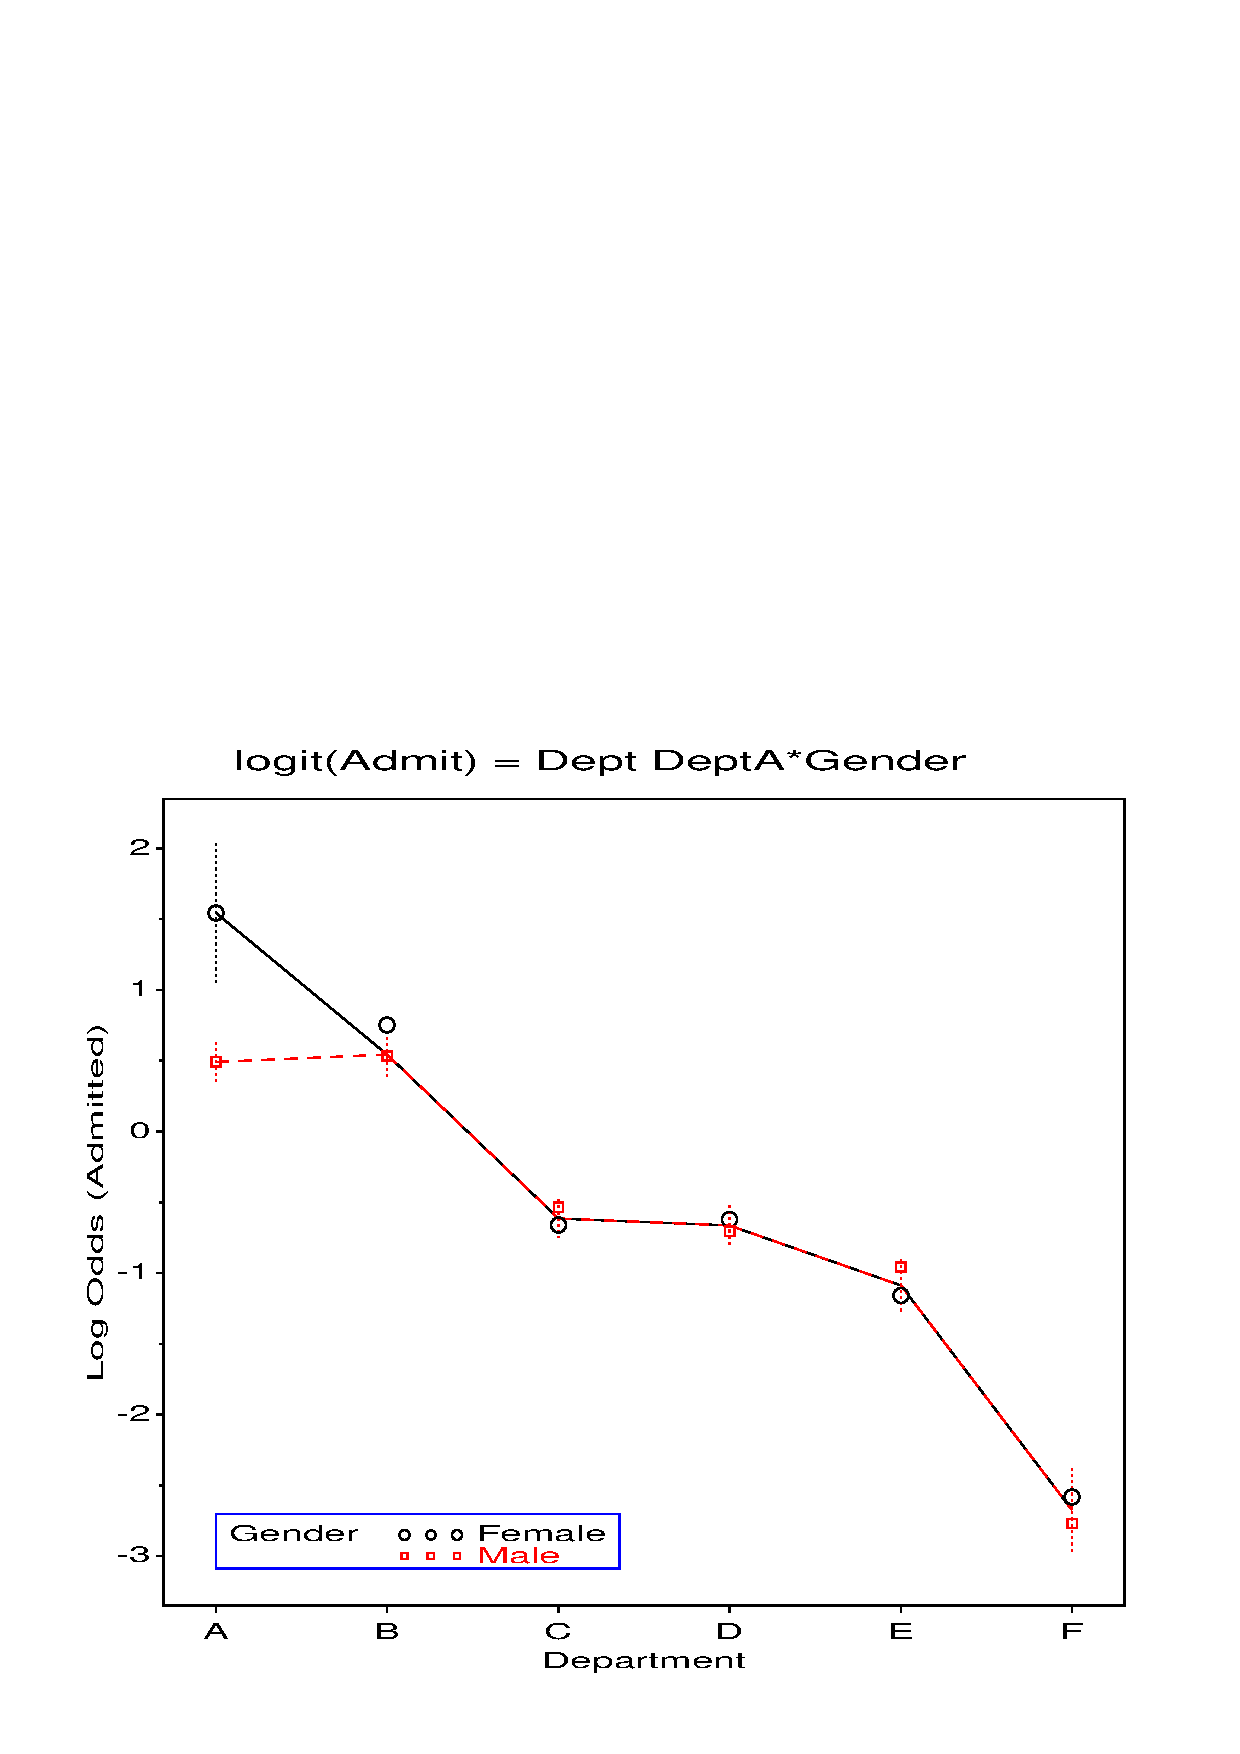
\includegraphics[scale=.6]{catberk6}
  \caption{Observed and fitted logits for model \eqref{eq:berk2}}%
  \label{fig:catberk6}
\end{figure}
The resulting plot for this model is shown in \figref{fig:catberk6}.
The graph gives a visual interpretation of the model
\eqref{eq:berk2} and its logit form, \eqref{eq:berk4}:
No effect of gender on admission, except in department A, where the
extra parameter allows perfect fit.
\end{Example}
